\section{Analyse}
        
    
    \subsection{Kravliste}
        \begin{enumerate}
            \item Spillet skal være mellem 2 - 4 personer
            \item Spillerne skal slå terninger på skift
            \item Der skal udskrives en tekst der omhandler det aktuelle felt, når spilleren lander på et felt
            \item Hver felt skal have en effekt for spilleren
            \item Spillerne starter med en balance på 30.000
            %Efter de nye regler så starter spillerne med hhv. 20, 18 eller 16 Matadollars, alt efter om der er 2, 3 eller 4 spillere.
            \item Spillet slutter når alle undtagen en spiller er bankerot, altså når deres balance er nået 0
            %Efter de nye regler så er der når den første spille går bankerot
            \item Spillerne skal kunne gå flere omgange rundt på spillepladen
            \item Spillet skal kunne kører på DTU’s databarer
        \end{enumerate}

%---------------------------------------------------------------------------
%                             Input af usecases
%--------------------------------------------------------------------------
\input{UseCases.tex}

\pagebreak
\subsection{UseCase diagram}
    \begin{figure}[h]
        \advance\leftskip-3cm
        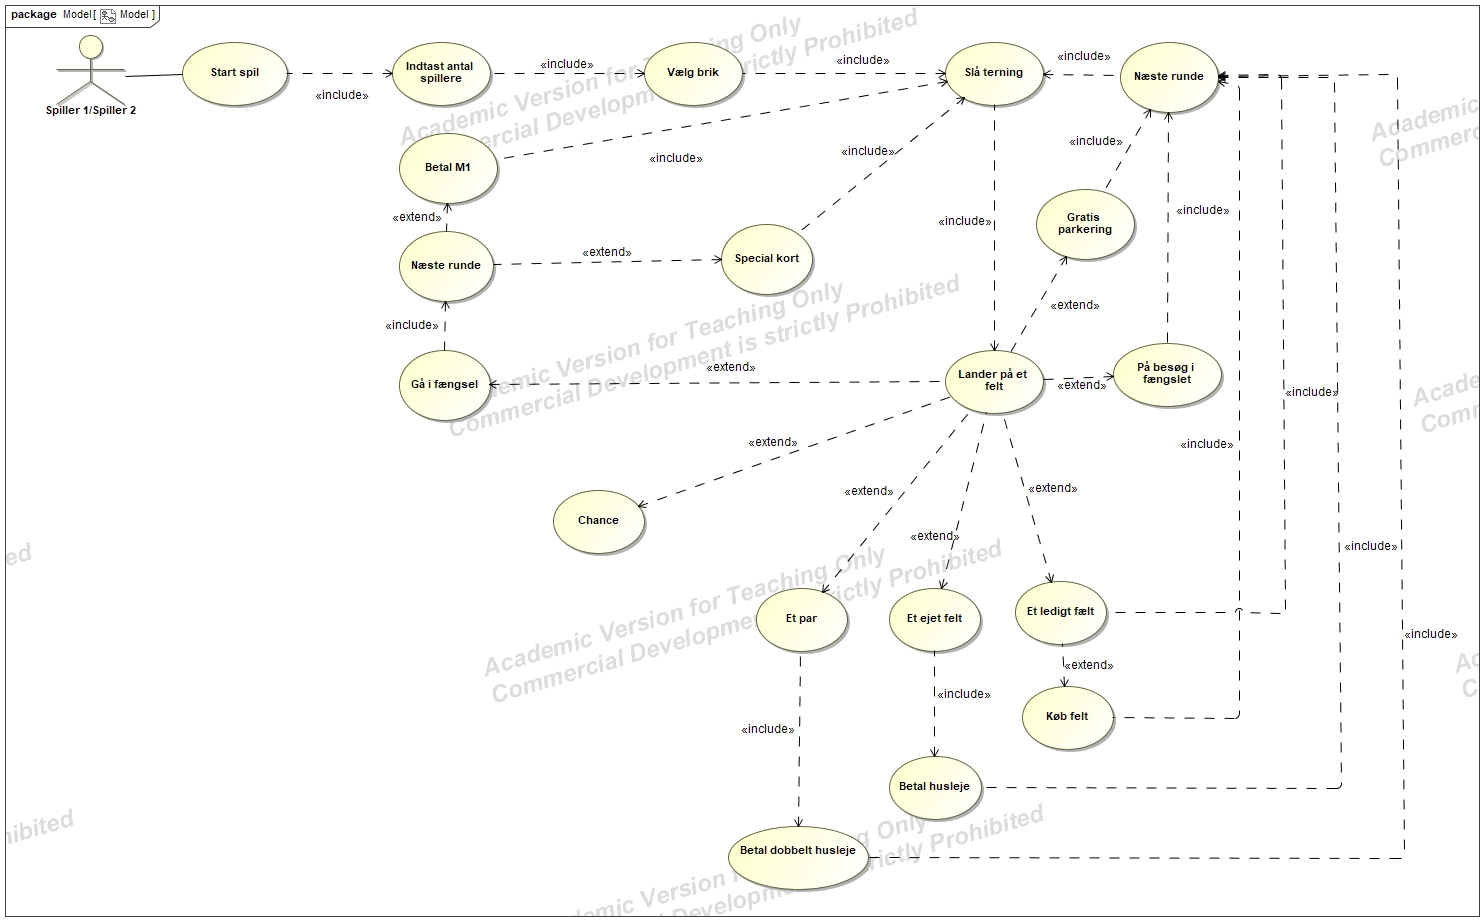
\includegraphics[width=20cm]{fig/UC-cdio3.jpg}
        \caption{UseCase diagram tegnet i MagicDraw}
    \end{figure}

\subsection{GRASP}
    GRASP står for General Responsibility Assignment Software Patterns. GRASP bruges til at give det rigtige ansvar til de forskellige klasser der bliver oprettet under udviklingen af et program. GRASP indeholder 9 patterns. Patterns bliver brugt til at strukturere et problem, samt at finde en passende løsning. De 9 patterns er:
        \begin{enumerate}
            \item Creator
            \item Information expert
            \item Low coupling
            \item Controller
            \item High cohesion
            \item Indirection
            \item Polymorphism
            \item Protected variations
            \item Pure fabrication
        \end{enumerate}
    (Der skrives mere når vi er nået længere i projektet)
